%%%%%%%%%%%%%%%%%%%%%%%%%%%%%%%%%%%%%%%%%%%%%%%%%%%%%%%%%%%%%%%%%%%%%%%%%%
%%%%%%%%%%%%   CAPTER 1   %%%%%%%%%%%%%%%%%%%%%%%%%%%%%%%%%%%%%%%%%%%%%%%%
%%%%%%%%%%%%%%%%%%%%%%%%%%%%%%%%%%%%%%%%%%%%%%%%%%%%%%%%%%%%%%%%%%%%%%%%%%
\chapter{Introduction}
\label{chap:introduction}

%%%%%%%%%%%%%%%%%%%%%%%%%%%%%%%%%%%%%
%%%%%%%%%%%%%%%%%%%%%%%%%%%%%%%%%%%%%
%%%%%%%%%%%%   SECTION   %%%%%%%%%%%%
%%%%%%%%%%%%%%%%%%%%%%%%%%%%%%%%%%%%%
%%%%%%%%%%%%%%%%%%%%%%%%%%%%%%%%%%%%%
\section{Radar Introduction}
\label{sec:intro:radarintroduction}
RADAR stands for RAdio Detection And Ranging. It is intended to detect and locate objects such as aircraft, motor bike, missiles, etc. Radar works the same way as how Bats navigate in the dark. But, instead of ultrasonic sound waves, Radar uses electromagnetic waves, that can travel long distance. The Radar sends an electromagnetic wave to a target, then analyses the echo from the target to determine target's information like position, velocity. Applications of Radar are spanned in many areas of engineering. It includes ultra-wide Band radar for human body monitoring and imaging \cite{radarMedi}, early warning system in military applications, measuring sea level, wave direction in remote sensing and lot more. Weather applications, precipitation animation in smart phones and weather forecast are some of the use cases of weather Radar. Pre-Collision System and Advanced Driver Assistance System in automobile are using Radars to detect imminent collision as well as takes mitigation plan \cite{radarCollAvoid}.

\subsection{Principle of Radar}
\label{sec:intro:principleofradar}
Radar can be classified as Pulsed Radar or Continuous Wave Radar based on the operating principle. Pulsed Radar, also called Pulse Doppler Radar, sends a short pulse then waits for the echo. The received echo is processed alongside. Pulse Doppler Radar is widely used in military applications. It has an antenna that acts as a transmitter and receiver. A short duration high energy pulse is generated and transmitted through the antenna. Up to this point, the antenna acts as a transmitter. As soon as the pulse is released from the transmitter, it is switched to receiver mode and is listening for echo from the target. Figures \ref{fig:intro:radar:blockdia} and \ref{fig:intro:radar:txrx} illustrate the block diagrams of the pulse doppler Radar and target detection respectively. The Continuous Wave Radar, as the name suggests, transmits electromagnetic signal continuously and the received echoes are processed.

\begin{figure}[h!]
	\centering
	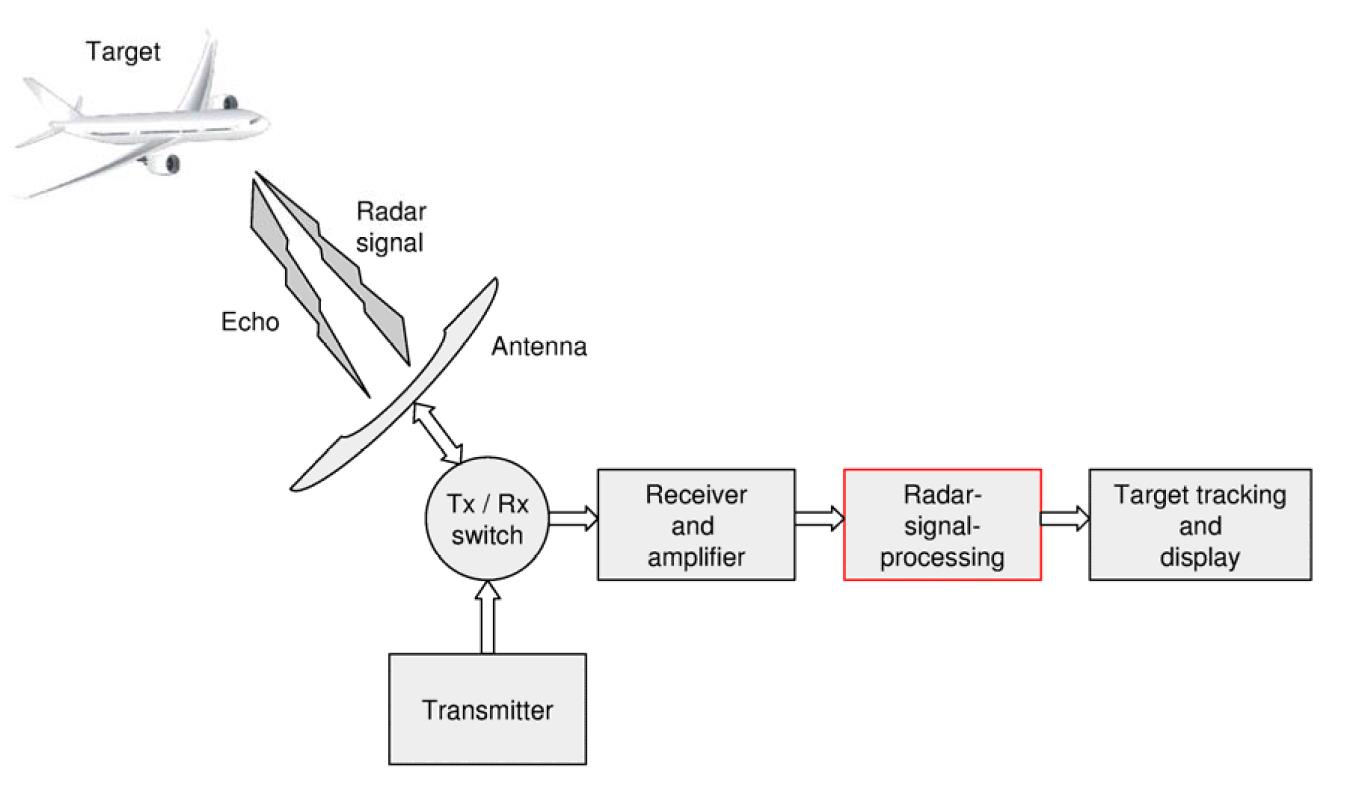
\includegraphics[width=130mm, height=75mm]{figures/radar_principle}
	\caption{Block Diagram of Pulse Doppler Radar \cite{Ludl}}
	\label{fig:intro:radar:blockdia}
\end{figure}

The time delay between sending the pulse and receiving the echo reveals the distance to the target. The frequency shift in the echo tells the radial velocity of the target.
\begin{figure}[h!]
	\centering
	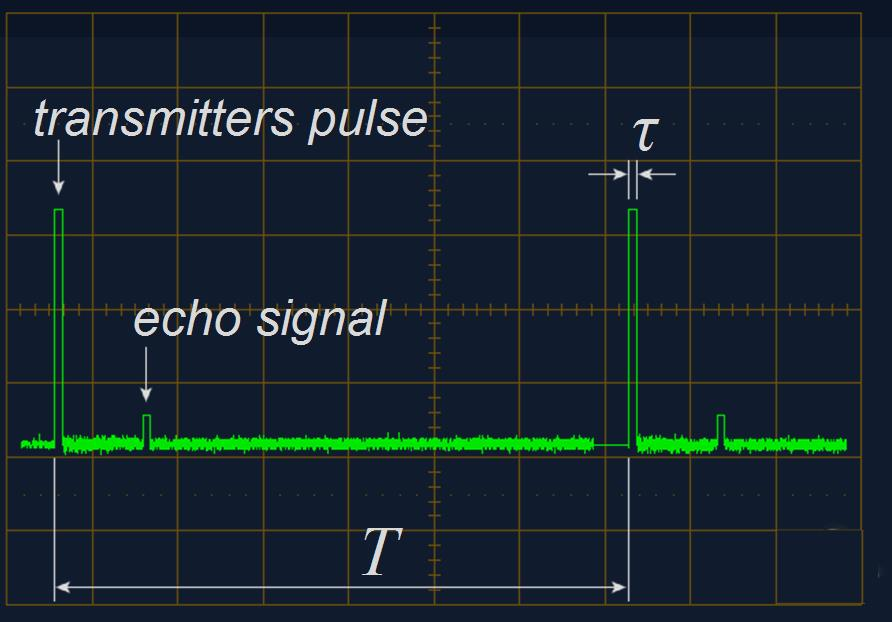
\includegraphics[width=75mm]{figures/trRx}
	\caption{Transmitter's Pulse and Echo Signal from Target \cite{radarTut}}
	\label{fig:intro:radar:txrx}
\end{figure}

Conventional waveband format is followed by manufacturers to address the radar operating frequency. Nowadays, radars are operated from 300MHz to 100GHz in different wavebands. The purpose and installation location of the radar determines the waveband. The accuracy of the radar is proportional to the operating frequency. Also, high frequency signals are more attenuated to water droplets and water vapours in the atmosphere. On the other hand, attenuation of the lower frequency signals is lower than high frequency signals. The typical use case of low frequency radar is in Early Warning Systems whereas high frequency radars are deployed in missile guidance systems \cite{radarExample}.

\subsection{Terminologies}
Radar systems use the spherical coordinate system to localize an object in the sky. The three following information are required to pin point an object relative to the Radar's position.

\textsl{\textbf{Azimuth angle ($\theta _{az}$):}} It is the angle between north and the target in horizontal plane. Azimuth angle can say whether the target is in the left side or right side to the north.

\textsl{\textbf{Elevation angle ($\varphi _{el}$):}} It is the angle between the target and Radar's local plane. Elevation says altitude of the target relative to the Radar. The Azimuth angle and Elevation angle of the Sun are explained in Figure \ref{fig:intro:radar:aziele}.

\textsl{\textbf{Radial distance (r):}} Distance between the target and Radar.\\

\begin{figure}[h!]
	\centering
	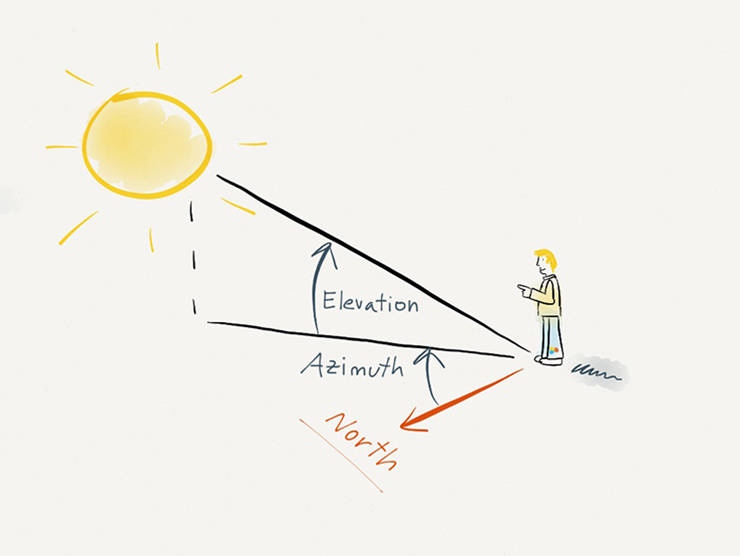
\includegraphics[width=75mm]{figures/azimuth_elevation}
	\caption{Azimuth and Elevation of the Sun \cite{aziEle}}
	\label{fig:intro:radar:aziele}
\end{figure}
\noindent
Other terminologies related to this thesis are explained here. \\[0.4cm]
\textsl{\textbf{Pulse:}} The Radar transmits an electromagnetic signal for a short duration (T$_{on}$) called pulse, then a break (T$_{off}$) follows to receive the echo of the pulse. This T$_{on}$ and T$_{off}$ together is called Pulse Repetition Time (PRT). Actual frequency of the electromagnetic wave transmitted during T$_{on}$ period is called carrier frequency.\\[0.2cm]
%\vspace*{0.2cm}
\noindent
\textsl{\textbf{Burst:}} The Radar sends $n$ number of pulses and listens to the echo signal. The combination of the selected PRT and the number of pulses are called Burst. Figure \ref{fig:intro:radar:prf} shows two different bursts having 3 pulse count each.

\begin{figure}[h!]
	\centering
	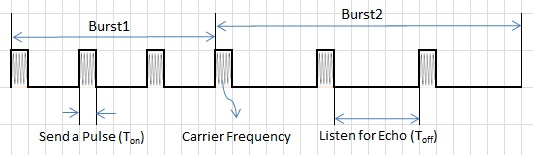
\includegraphics[]{figures/prf}
	\caption{Example of Burst}
	\label{fig:intro:radar:prf}
\end{figure}
\vspace*{0.2cm}
\noindent
\textsl{\textbf{PRF:}} Inverse of Pulse Repetition Time is called Pulse Repetition Frequency. \\
\noindent
\textsl{\textbf{Dwell:}} Group of 8 different bursts form a dwell.
\FloatBarrier

%%%%%%%%%%%%%%%%%%%%%%%%%%%%%%%%%%%%%
%%%%%%%%%%%%%%%%%%%%%%%%%%%%%%%%%%%%%
%%%%%%%%%%%%   SECTION   %%%%%%%%%%%%
%%%%%%%%%%%%%%%%%%%%%%%%%%%%%%%%%%%%%
%%%%%%%%%%%%%%%%%%%%%%%%%%%%%%%%%%%%%
\section{Motivation}
\label{sec:intro:motivation}
Radar is one of the core components of a combat air system. Range and accuracy of the Radar are important for missile system, guidance system, early warning system, etc. Massively parallel processor arrays, DSP processors, FPGA processors and GPU processors\cite{HalmSwe} are some examples of the Radar processors in the industry.  They demand high computation capabilities, more power and so big in size.

Avionics and military applications always thrives to minimize the Size, Weight and Power (SwaP) while demanding high performance. It remains the backbone of the research. This thesis explores the possibilities of bringing a new dimension to the low cost and real-time Radar processor that can be employed in safety critical systems. ARM processor, which is running in millions of smart devices\cite{armWeb} is chosen, keeping compactness, portability and power requirements in mind. As a first step, medium range (40nm) Radars are considered as a suitable candidates to adopt low cost and compact ARM processors, since they do not need several TFLOP of processing power to adhere the real-time requirements.

A baseline analysis is carried out by Airbus DS concludes that the ARM processors cannot meet the real-time requirements, if the scheduling of the Radar processing algorithm not optimized. This thesis extends the baseline analysis and implements a couple of optimized scheduling schemes to meet the real-time requirements. The results of the optimized schemes and possible improvements are discussed in detail.

%%%%%%%%%%%%%%%%%%%%%%%%%%%%%%%%%%%%%
%%%%%%%%%%%%%%%%%%%%%%%%%%%%%%%%%%%%%
%%%%%%%%%%%%   SECTION   %%%%%%%%%%%%
%%%%%%%%%%%%%%%%%%%%%%%%%%%%%%%%%%%%%
%%%%%%%%%%%%%%%%%%%%%%%%%%%%%%%%%%%%%
\section{Requirements of the Radar Processor}
\label{sec:intro:realtime_req}
A Radar mounted on an Aircraft or Satellite is called Airborne Radar. The Airborne Radar processor should be able to process Air to Air (A/A) Mode data and Air to Ground Mode (A/G) data. As the Radar processor is a part of a safety critical system, it should stick to the industrial standards DO-178B/C, ARINC-653.

Since this research is in the early stage of development, and to allow room for further requirements, the CPU utilization is restricted to 50\% of the available CPU time, memory utilization should be less than 50\% of the available memory size and the peak data transfer rate of the Radar application should be less than 50\% of the maximum achievable data transfer bandwidth. The real-time requirements of the Radar processor shall be summarized as follows
\begin{itemize}
        \itemsep0em
        \item \textit{Resulting processing latency:} The time span between reception of an echo and the processed information is sent out, should be less then 2x dwell time.
        \item \textit{Memory transfer bandwidth:} <50\%.
        \item \textit{Memory utilization:} <50\%.
        \item \textit{CPU utilization:} <50\%.
\end{itemize}


%%%%%%%%%%%%%%%%%%%%%%%%%%%%%%%%%%%%%
%%%%%%%%%%%%%%%%%%%%%%%%%%%%%%%%%%%%%
%%%%%%%%%%%%   SECTION   %%%%%%%%%%%%
%%%%%%%%%%%%%%%%%%%%%%%%%%%%%%%%%%%%%
%%%%%%%%%%%%%%%%%%%%%%%%%%%%%%%%%%%%%
\section{Problem Statement}
\label{sec:intro:probstatement}
The Airborne Radar is subjected to operate on different Pulse Repetition Frequencies (PRF) to resolve ambiguity in distance and velocity. Consecutive eight different bursts form a dwell. That is, on every time the Radar probes the sky, it sends one dwell and the echoes are received and analysed. The resulting processing latency of the baseline analysis is theoretically calculated as 15x dwell time (see Table \ref{tbl:mm:scheme1_true_latency}).  It means, to produce the result of the first dwell, it needs as much time as the 15 dwell transmission require. A typical dwell time is 54ms. An Eurofighter Typhoon moving at a speed of Mach 2 would move a distance of 560 meters during this processing time. Half a kilometer difference between detection and display is very high for a typical Airborne Radar processor.

The real-time requirement confines the processing latency to 2x dwell time. The investigation of this thesis is to find an optimal scheduling scheme, number of processors required, data distribution, resulting processing latency and exploit the parallelism in the Radar processing algorithm to stick to the real-time requirements.

%%%%%%%%%%%%%%%%%%%%%%%%%%%%%%%%%%%%%
%%%%%%%%%%%%%%%%%%%%%%%%%%%%%%%%%%%%%
%%%%%%%%%%%%   SECTION   %%%%%%%%%%%%
%%%%%%%%%%%%%%%%%%%%%%%%%%%%%%%%%%%%%
%%%%%%%%%%%%%%%%%%%%%%%%%%%%%%%%%%%%%
\section{Contributions}
\label{sec:intro:contrib}
One of the major works of this thesis is, binding the performance critical functional blocks of the Radar processing algorithm, to replicate the Radar processing chain, targeting multi-core architecture and multi-threaded application. In summary, the main contributions of this thesis are:

\pagebreak
\begin{itemize}
\item{\bf Multi-core Performance}
  \begin{itemize}
    \item Scalability and performance of the application on multi-core environment are estimated. Shared resources, resource contention and race condition are considered.
    \item All the threads are set to execute the functional blocks simultaneously to ensure the maximum memory transfer bandwidth.
  \end{itemize}
\item {\bf Scheduling Scheme}
 	\begin{itemize}
 	\item Data dependencies are identified and evaluated by executing them in parallel using POSIX Threads.
   	\item Constraints on non-thread-safe functional blocks are identified and scheduled them without violation.
   	\item Optimal scheduling schemes are proposed and their results are assessed.
	\end{itemize}
\item {\bf Measurement Tools}
  \begin{itemize}
      \item Developed automated scripts to measure peak memory utilization, CPU utilization, memory transfer bandwidth and processing latency.
  \end{itemize}
 \item {\bf Verification of Results}
   \begin{itemize}
       \item Results of multi core application are verified against the single core application.
   \end{itemize}
\end{itemize}

%%%%%%%%%%%%%%%%%%%%%%%%%%%%%%%%%%%%%
%%%%%%%%%%%%%%%%%%%%%%%%%%%%%%%%%%%%%
%%%%%%%%%%%%   SECTION   %%%%%%%%%%%%
%%%%%%%%%%%%%%%%%%%%%%%%%%%%%%%%%%%%%
%%%%%%%%%%%%%%%%%%%%%%%%%%%%%%%%%%%%%
\section{Thesis Outline}
\label{sec:intro:outline}

The rest of this thesis is organized as follows:

%\begin{compactitem}
\begin{itemize}
	\item \textbf{Chapter \ref{chap:bg_related_work}:} Explains the Integrated Modular Avionics (IMA) architecture, experimental set-up and related work concerning ARM processors in Radar application.

	\item \textbf{Chapter \ref{chap:existing_analysis}:} Discusses the results of the baseline analysis done by Airbus Defence and Space GmbH.

	\item \textbf{Chapter \ref{chap:testbed}} Explains the pros and cons of the baseline analysis, test bed information and important design choices.

	\item \textbf{Chapter \ref{chap:mode_mapping}:}  Proposes optimized scheduling schemes and verifies their correctness via implementation. Results of the new schemes are discussed.

	\item \textbf{Chapter \ref{chap:conclusion}:} Summarizes this thesis with a conclusion and proposes future work regarding the optimized schemes.
\end{itemize}
%

